\chapter{Crab Giant Pulses} \label{chap:crabpulsar}

This chapter outlines the analysis of over 6 years observations from Crab pulsar observed with I-LOFAR. The content closely follows that of \cite{Johnson2026Crab} which will be shortly submitted to the open journal of astrophysics for review. Some minor edits and expansion on jargon has been made for readability purposes. 

\section{Introduction}
The Crab Pulsar (PSR~B0531$+$21) is one of the most notable and well-studied pulsars, owing to its well-determined, relatively young age and its exceptional brightness. Embedded at the centre of the Crab Nebula, the pulsar is the remnant of the historical supernova of 1054 CE with radio emission first noted in 1968~\citep{sr68}. The pulsar provides a unique opportunity to investigate both the physics of neutron stars and the dynamics of supernova remnants. The Crab emits strongly across the entire electromagnetic spectrum, making it an invaluable tool for studying the interaction between a pulsar and its surrounding nebula \citep{hester_crab_2008}.

Due to its brightness and dynamic environment, the Crab Pulsar is also an excellent source for studying emission and probing the free-electron content of the surrounding nebula. At frequencies below 300 MHz, dispersion measure and scattering effects become particularly pronounced, and these effects have been observed consistently for decades in the Crab system~\citep{lyne_23_1993}. The evolving nebula causes time dependant propagation effects on monthly to yearly timescales. This work details over half a decade of low-frequency observations of the Crab pulsar and present the largest collection of single pulses from the Crab to date. 

This work is structured as follows: \cref{sec:bkginfo} provides the scientific context and motivation for this study; \cref{sec:obsnmethod} describes the observations and methodology used for pulse detection and analysis; and \cref{sec:results} presents a statistical overview of the giant-pulse population and examines DM variations and scattering timescales; Finally, \cref{sec:results} gives concluding remarks and potential future work on the topic. 

\section{Background \& Motivation} \label{sec:bkginfo}

\subsection{Giant Pulses}
The pulse amplitude distribution of the Crab pulsar is broad~\citep{hje15}. The brightest pulses are referred to as ``giant pulses'' (GPs). The working definition of GPs isn't consistent throughout the literature but for this work it is considered to be pulses that are brighter than ten standard deviations above the noise floor. GPs from the Crab pulsar are sporadic, their durations range from as long as milliseconds to as low as being unresolved down to picoseconds retaining their coherence \citep{jessner_giant_2010,thulasiram_narrow-band_2021}. GPs have also been noted to show narrowband features as consequence of the Heisenberg-Gabor limit \citep{bij_kinematics_2021}. The peak flux density of a GP ranges from $10^{3}-10^{5}$ Jy~\citep{thulasiram_narrow-band_2021}, and they closely follow a power-law distribution of, $N(F)\propto F^\alpha$ where $\alpha$ ranges from $-1.5$ to $-3.6$, depending on pulse phase~\citep{sokolowski_100_2025, karuppusamy_giant_2010}. This indicates that these bright pulses are not exceedingly rare. The power-law distribution extends across three orders of magnitude in fluence, with no evidence of a high fluence cut-off. 

One of the most noteworthy things about GPs is their brightness temperature. Single pulses can reach temperatures of at least $10^{32}~\rm K$ in observations that do not resolve the finest temporal structure, and are known to reach $10^{37}~\rm K$ in nanosecond-resolution observations \citep{cordes_brightest_2004}. This places GPs as some of the brightest signals in the observable Universe. Observation of giant pulses exhibit significant variability with detection rates measured from 100 -- 3000 pulses per hour. Intervals of lower and higher intensity activity show that the successive detections exhibit a Poisson distribution \citep{sokolowski_100_2025}.

\subsection{The Crab Nebula}
The Crab Nebula has a stratified structure, at its core lies the Crab surrounded by relativistic magnetized wind flowing outward~\citep{lyubarsky_structure_2002}. This wind interacts with a termination shock, a boundary region where the wind's kinetic energy is converted into heated plasma and magnetic compression \citep{lyubarsky_structure_2002, gaensler_evolution_2006}. The shocked wind forms a synchrotron-emitting nebular interior composed of electrons, positrons, and wound-up magnetic fields \citep{hester_crab_2008}. Beyond this inner region, the synchrotron nebula expands into supernova ejecta. This ejecta has cooled and condensed into regions made up primarily of ionized oxygen, forming a network of structures visible at optical wavelengths \citep{hester_crab_2008}. The filamentary structure exhibits both large-scale organization and small-scale turbulence, with the pulsar wind continuously pushing against these thermal structures creating a dynamic environment \citep{hester_crab_2008}.

Of most relevance for our work we note that the Crab Nebula contains a substantial population of free electrons distributed throughout all three regions, the wind, shocked nebular interior and the ejecta filaments \citep{kuzmin_deviation_2008}. Within the nebula the average electron number density is $\Delta n_e \sim 0.018~\rm{cm}^{-3}$ and this results in a dispersion measure contribution $\Delta \mathrm{DM} \sim 0.03~\rm{cm}^{-3}$ when using a nebula radius of 1.7 pc \citep{kuzmin_deviation_2008, mckee_temporal_2018, hester_crab_2008}. 


\subsection{Probing the Free Electron Content}

% Dispersion Measure (DM) measures the total column density of free electrons encountered by radio waves on the way to the observer, expressed as $\text{DM} =\int n_e \ dl$. DM causes a time delay in the arrival of the radio wave based on its frequency, which can be expressed as $\Delta t = \text{DM}/(\mathcal{D}\nu^2)$. Where $\mathcal{D \simeq}~2.41\times10^{-4}~\text{MHz}^{-2}$ known as the dispersion constant and $\nu$ is the observing frequency.  

Because dispersive delay scales as $\Delta t\propto\text{DM}\nu^{-2}$ at low frequencies the delay is much more pronounced, making it easier to measure DM precisely. This makes telescopes like the LOw Frequency ARay \citep[LOFAR;][]{van_haarlem_lofar_2013} one of the best instruments for determining DM, long timing campaigns routinely achieve DM uncertainties on the order of $10^{-5}$\dm \citep{iraci_pulsar_2024}. The exceptional brightness of GPs means that with a LOFAR international station residual smearing can be accounted for making GPs a highly sensitive probe of small DM offsets and short-timescale variations.

The Crab Pulsar is noted to have a DM of 56.7712(3) \dm according to ATNF catalogue \citep{ATNFCat_2005}. However, this value is not static, it's been noted to have temporal variations on timescales of weeks to years on scales of $\pm0.01-0.15$\dm \citep{lyne_23_1993}. These variations indicate a change in electron density along the line of sight to the Crab pulsar and can be used as tracers for the surrounding nebula \citep{isaacman_crab_1977}. In addition to this, there is also a contribution from the turbulence in the interstellar medium and the solar wind. 

% \subsection{The Solar Wind}

The Sun continuously emits a magnetised plasma outflow, known as the solar wind, which fills the heliosphere with free electrons. Consequently, this can affect radio waves in any line of sight in the inner solar system \citep{tiburzi_impact_2021}. Any pulsar signal observed near the ecliptic plane can thus be impacted by the contribution of the solar wind. This is commonly modelled as $n\propto r^{-2}$ but in practice the structure vary with heliographic latitude, longitude, and solar cycle \citep{susarla_exploring_2024}. The contribution of the solar wind manifests in measurements by adding variations on scales of $10^{-4}$~\dm. 

\section{Observations \& Methods} \label{sec:obsnmethod}

\subsection{Observations} 

Observations were taken using the Irish LOw Frequency ARray station (I-LOFAR) using the REALTA backend \citep{RealTa_paper} for processing. Observations were taken over a time range from June 2020 to March 2026 totalling $\tobs$ hours and covering $\epochs$ epochs as shown in \cref{fig:crab_sun_seperation}. The High Band Antennas were used for each of the observations, which observed from $\approx 102-198$~MHz. During observations, UDP packets of beam-formed data are written to disk. The saved data are made up of coarse-channelized complex voltages.  The input data stream consists of two polarizations per antenna. After real Nyquist sampling with a 200-MHz clock and coarse channelization by a factor of 512, only 488 channels (or 244 channels) are recordable when the data is written as 8-bit (or 16-bit) complex samples, for this study 8-bit mode is used. The \textsc{udpPacketManager} \citep{David_JOSS} is then used to create \textsc{sigproc} \citep{lorimer_sigproc_2011} formatted filterbanks at the specifications detailed in \cref{tab:data_details}

\begin{table}[h]
    \centering

    \begin{tabular}{lc}
        \hline
        \textbf{Data Attribute} & \textbf{Value} \\
        \hline
        Frequency Start $(f_\text{start})$ & 102.234131 MHz \\
        Frequency End $(f_\text{end})$ & 197.546387 MHz \\
        Frequency Resolution & $24.4414\,\mathrm{kHz}$ \\
        Temporal Resolution & $655.36\,\upmu\mathrm{s}$ \\
        \hline
    \end{tabular}
    \caption[Crab data sepecifications]{Specifications of data as generated with \textsc{udpPacketManager}~\citep{David_JOSS}.}
    \label{tab:data_details}
\end{table}


\begin{figure}[t]
    \centering
    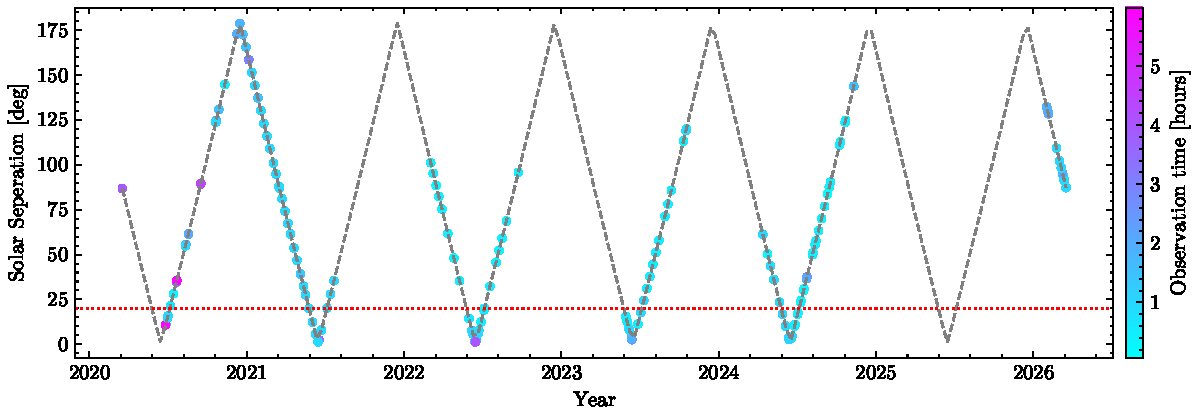
\includegraphics[width=0.94\linewidth]{chapter4/figures/crab_sun_separation.pdf}
    \caption[Observation epochs of the Crab with I-LOFAR]{Each of the \epochs\ epochs covering a total of \tobs\ hours over 6 years of data plotted against solar separation.}
    \label{fig:crab_sun_seperation}
\end{figure}

\subsection{Identifying Pulses}

The first step in analysing these data is the identification of bright single pulses; this is done using \textsc{transientX}~\citep{men_transientx_2024}. 
%which provided a list of single pulses and also excised Radio Frequency Interference (RFI). 
Single pulses with widths of $5-50$~ms were searched for to generate candidate lists for each epoch, 5~ms was chosen due to ISM scattering at the low end of the band being $\sim6.32~\mathrm{ms}$ (see \cref{appen:low-frequency-dd}). To reduce computational cost, the search was performed on 8-bit filterbanks rather than 32-bit. The candidate lists provide time-stamps used to extract portions of the 32-bit filterbanks. For each burst where an S/N of $>100$ was measured, a \textsc{psrchive} \citep{hotan_psrchive_2004} single-pulse archive file was generated, where $t_{\rm start} =  t_{\rm burst}- 3.276~\rm ms$ and $t_{\rm end} =  t_{\rm burst}+ 32.768~\rm ms$. This window was chosen such that the single-pulse filterbanks didn't include multiple rotations and the sample start time was 10\% of a rotation before the burst recorded burst time. The brightest pulse in the dataset was found to have an S/N of 7214 and is shown in \cref{fig:joy_division}, this is a prime example of the benefit of observing GPs at low frequency as the scattering is easily observed in each of the sub-bands.  


\begin{figure}
    \centering
    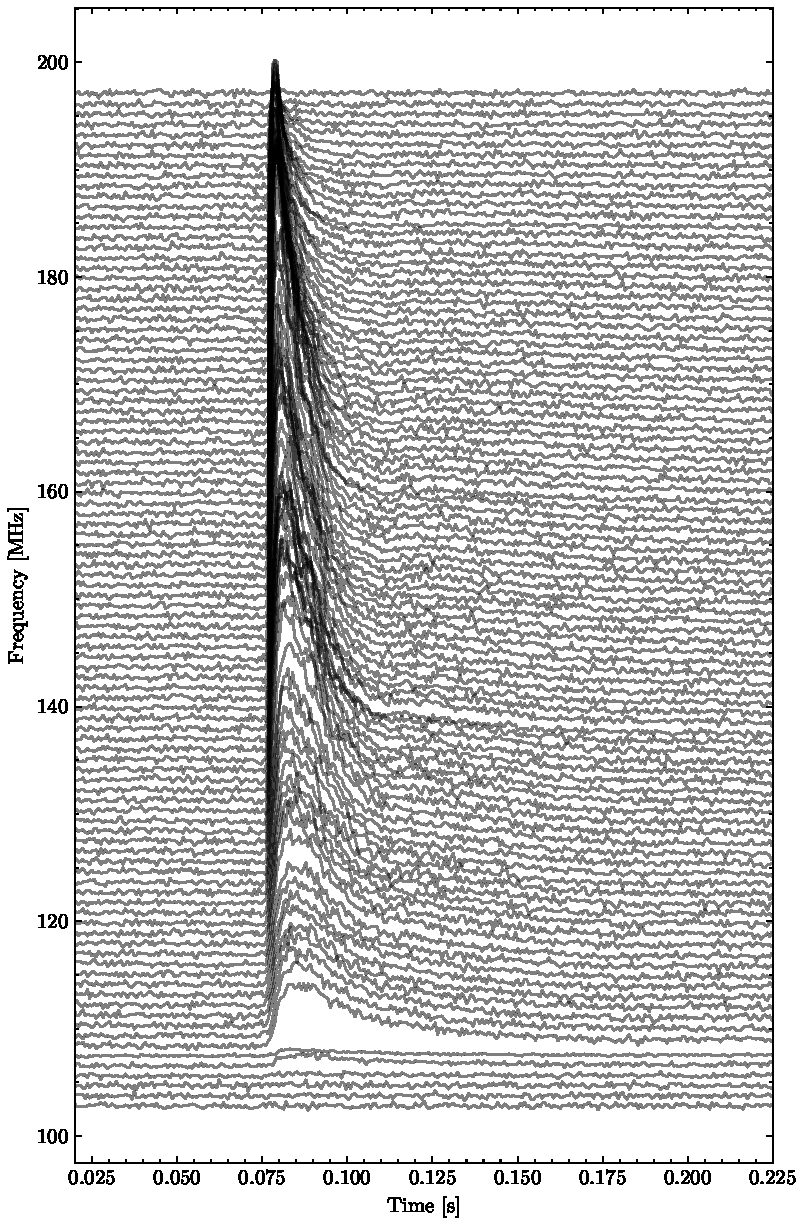
\includegraphics[width=0.9\linewidth]{chapter4/figures/joy_div.pdf}
    \caption[Joy division plot of Crab Giant Pulse]{Waterfall plot of the brightest giant pulse across all epochs. The burst was observed at 2023-10-17T04:33:38.896 with a corrected DM of $56.754 \pm 0.002$ \dm~ and an S/N of 7214.}
    % Loading /mnt/ucc4_data2/data/filterbanks/Crab/2023-10-17/transientx_output/Crab_60234.1900335157_cfbf00000_01_01.ar with DM 56.754279278705546 pm 0.0021658506908873096 and SNR 7214.0183283150
    \label{fig:joy_division}
\end{figure}

\subsection{Correcting the DM}

Due to the large amount of scattering present at lower frequency, traditional boxcar single-pulse searches can often over or underestimate the DM as they simply maximise S/N over a reasonably coarse search grid in DM and pulse width. An example of this is shown in \cref{fig:DMvariation}. The initial DM, from the \textsc{transientx} detection was corrected by using \textsc{DM\_phase} \citep{seymour_dm_phase_2019}, which optimises based on coherent radio power (phase of the pulse) across the band. This is done by ingesting RFI-cleaned archive files and dedispersing across a range of trial DMs. The trial DM that maximises inter-channel phase coherence, rather than the amplitude of the dedispersed time series, is selected. The corresponding dispersive delay, $\Delta t$ is applied. After dedispersion, the intensity waterfall $I(\nu_i,t)$ is Fourier transformed along the pulse phase/time axis to obtain $\tilde{I}_i(f)=\mathcal{F}_t\{I(\nu_i,t)\}$. The phase-only spectrum is then formed by normalising the amplitude like:
\begin{equation}
\hat{I}_i(f)=\frac{\tilde{I}_i(f)}{\left|\tilde{I}_i(f)\right|}\,.
\end{equation}
This is then summed coherently across all frequency channels like:
\begin{equation}
C(f;\mathrm{DM})=\sum_{i=1}^{N_\nu}\hat{I}_i(f), \qquad
P(f;\mathrm{DM})=\left|C(f;\mathrm{DM})\right|^2 \,.
\end{equation}
A one-dimensional DM metric is obtained by integrating $P(f;\mathrm{DM})$ over a range in fluctuation frequency $f$,
\begin{equation}
S(\mathrm{DM})=\sum_{f=f_{\rm low}}^{f_{\rm high}} w(f)\,P(f;\mathrm{DM})\,,
\end{equation}
and the best-fit DM is selected as the maximum $S(\text{DM})$. The DM uncertainty is estimated by fitting a polynomial to the peak of $S(\mathrm{DM})$ and using the curvature at the maximum (Hessian approximation) $\mathrm{DM}_0$, giving
\begin{equation}
\sigma_{\mathrm{DM}}=\sqrt{\left|\frac{2\,\varepsilon}{{S_{\text{max}}}''(\mathrm{DM}_0)}\right|}\, ,
\end{equation}
where $\varepsilon$ is a noise scale for the DM metric.

\begin{figure}
    \centering
    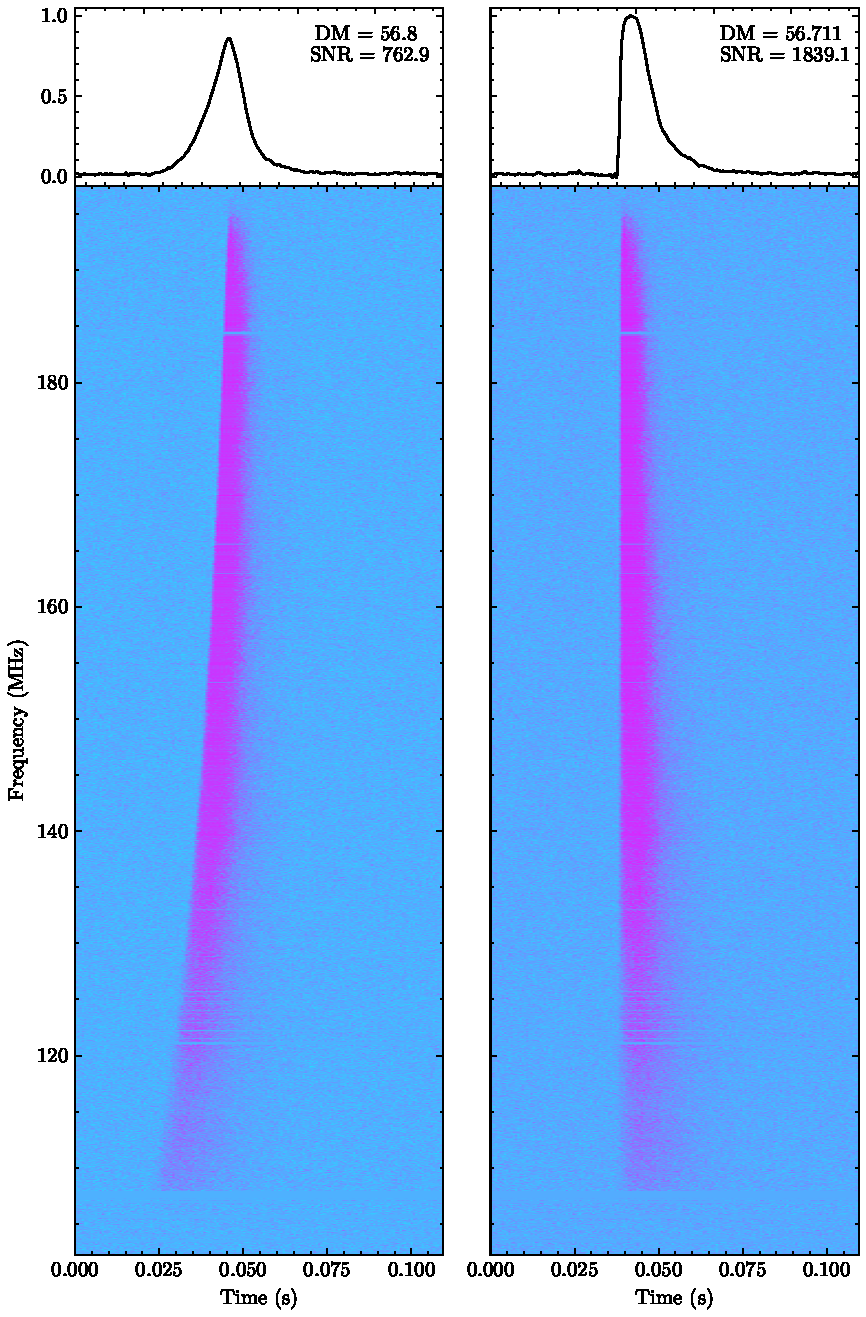
\includegraphics[width=0.9\linewidth]{chapter4/figures/DMcompare.pdf}
    \caption[\textsc{DM\_phase} giant pulse detection.]{The \textit{left} shows an example of a giant pulse where the initial DM guess that \textsc{transientX} founded by fitting a boxcar, the \textit{right} shows the phase corrected DM that was calculated by \textsc{DM\_phase}}
    \label{fig:DMvariation}
\end{figure}

\subsection{Modelling Scattering} \label{sec:modelScattering}

Previously outlined by  \citet[][pp.~208--220]{mckennathesis2023}  due to high precision that DM can be determined with a single international LOFAR station its possible to model the scattering of individual pulses as a function of frequency. Splitting pulses into 10~MHz chunks, three models have been previously used to model scattering time as a function of frequency and time \citep{bhat_detection_2007, karuppusamy_giant_2010}. 
The thin screen model proposed by \cite{bhat_clean-based_2003}, assumes that scattering occurs within a narrow layer located on an infinite plane. Because the screen is sufficiently thin, photons crossing it experience no change in propagation speed, and the observed delay arises purely from the geometric path difference caused by the scattering event. It is described as follows: 

\begin{equation}
    f_{\text{thin}}(t, t_0,\tau,A) = \frac{A}{t} \exp \left[ -\frac{t - t_0}{\tau} \right] H (t - t_0)
    \label{eq:thinmodel}.
\end{equation}

This models the pulse with an exponential decay with a characteristic value for scattering, $\tau$. Here $H(t-t_0)$ is a delayed Heaviside step function for an event that occurs at $t_0$. It switches the model on at $t>t_0$ and off for $t<t_0$. $A$ is then the amplitude used to scale to the pulse profiles if they are not normalised. Observationally this model did not fit at lower frequencies thus a modified version of the thin model was implemented by \cite{karuppusamy_giant_2010}. This modification added a scaling factor of $t^\gamma$ to better emulate the rise of the exponential peak observed. This is described by \cref{eq:thin_model_mod}, 

\begin{equation}
    f_{\text{mod, thin}} (t_, t_0, \tau, A, \gamma)= A(t-t_0)^\gamma \exp \left[ -\frac{t - t_0}{\tau} \right] H(t-t_0). 
    \label{eq:thin_model_mod}
\end{equation}

Similarly \cite{williamson_pulse_1972} describes a thick model. In the thick model photons are continuously scattered during their propagation from the source to observer through a fraction of the medium. In this case \cref{eq:thick_model} places the screen close to the source which can be used to model the effect of the Crab's nebula on individual pulses. 


\begin{equation}
    f_{\text{thick}} (t,t_0,\tau,A) = \sqrt{\frac{A \pi \tau}{4(t-t_0)^3}} \exp\left[ - \frac{\pi^2}{16(t-t_0)} \right] H(t -t_0)
    \label{eq:thick_model}
\end{equation}

For each of the that have been DM corrected the respective archive file is read and split into 9.53~MHz subbands (see \cref{fig:scattering}). Each subband is then fitted to both \cref{eq:thin_model_mod} and \cref{eq:thick_model} using \textsc{lmfit} to compute statistical significance of each fit in a number of ways. \Cref{eq:thinmodel} was omitted from fitting due to previous studies \citep{karuppusamy_giant_2010} and preliminary work on this data set \citep[][pp. 208--220]{mckenna_thesis_2023} as the model failed to converge with any of the subbands in this frequency range. 

\begin{figure}
    \centering
    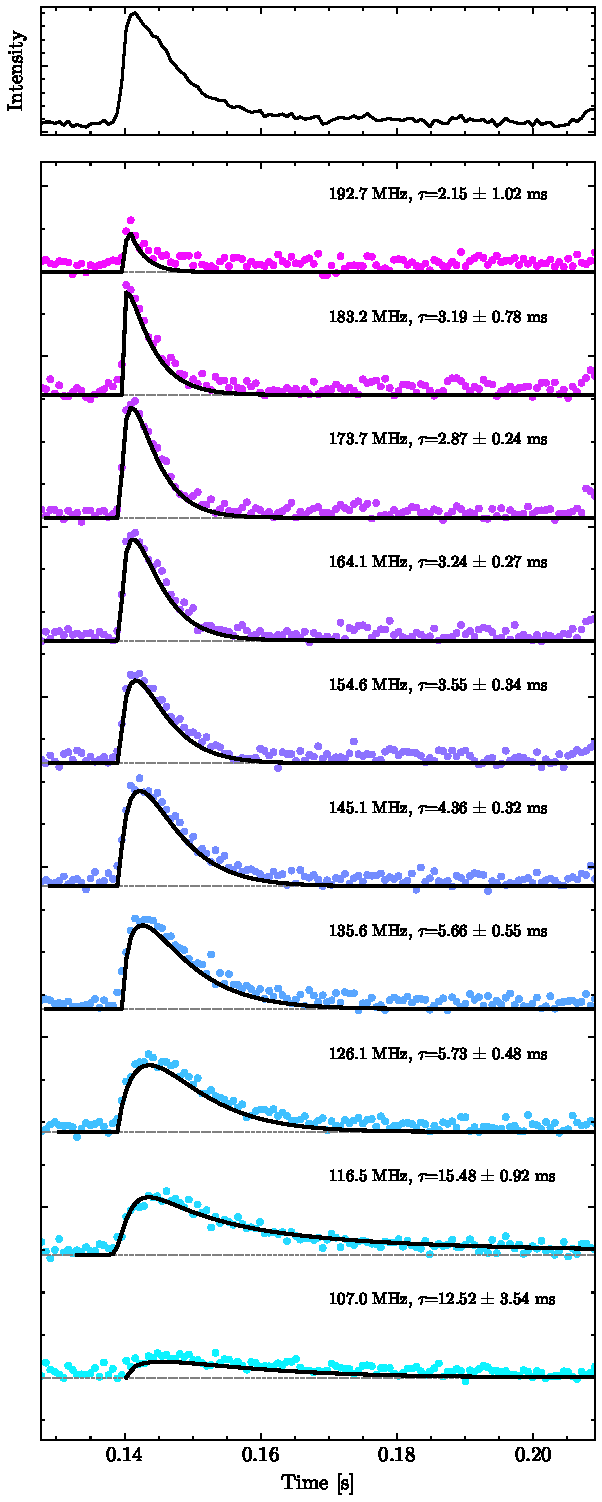
\includegraphics[width=0.58\linewidth]{chapter4/figures/Crab_scattering_fit.pdf}
    \caption[Example of pulse scattering across the LOFAR band]{Example of the scattering fits applied to an example giant pulse that has a post corrected SNR of 291. Here the black line represents the fitted scattering model, scatter points are the observed data. }
    \label{fig:scattering}
\end{figure}

\subsection{Folding}

In addition to the analysis of the Crab GPs, each of the epochs were also folded for a comparison. For each epoch the Crab ephemeris measured monthly by Jodrell bank was used\footnote{\url{https://www.jb.man.ac.uk/pulsar/crab/}} \citep{lyne_23_1993} as a first guess, \textsc{PRESTO} was then used to further refine DM and period values before timing with \textsc{TEMPO2} \citep{hobbs_tempo2_2006}. Initial efforts were made to time each epoch as described in \citet{iraci_pulsar_2024} and \citet{susarla_long-term_2025}, however determining an accurate for ephemeris for the Crab across over half decade proved difficult due to scattering exhibited in the Crabs pulse profile along with DM variations on short timescales (see. \cref{fig:foldedprofile}). DM was determined using single epoch timing values through the creation of a template from a high SNR observation and then fitting DM to from Time of Arrivals (TOAs) for 8 subbands in the archive. Due to the scattering the error was on the order of $10^{-2}$~\dm~for each of the epochs, whereas for other pulsars without complex scattering its on the order of $10^{-5}$~\dm~\citep{susarla_long-term_2025}. Due to this the folded analysis was omitted from the DM time series as it provided no further insights than its higher frequency contemporaries. 

\begin{figure}
    \centering
    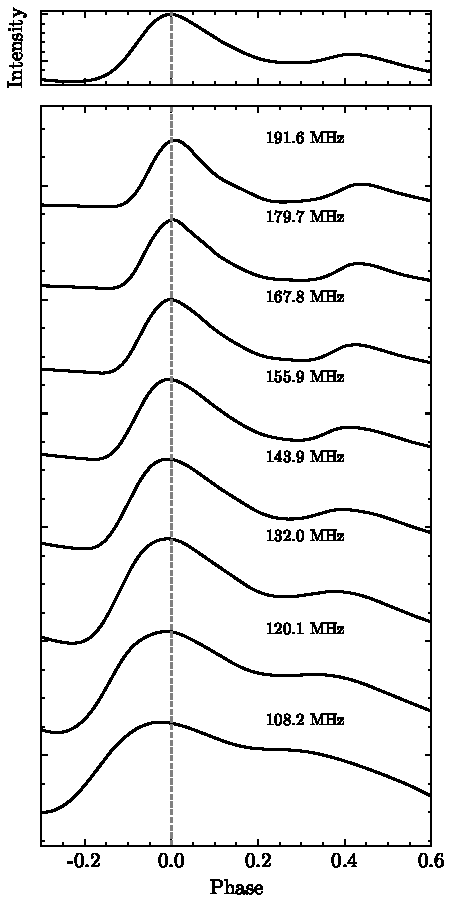
\includegraphics[width=0.7\linewidth]{chapter4/figures/template.std_subbands.pdf}
    \caption[Smoothed folded profile of the Crab]{Smoothed folded profile of a 2-hour observation taken on 2026-03-17. Split into 12~MHz chunks.}
    \label{fig:foldedprofile}
\end{figure}

\section{Results} \label{sec:results}

This work details the analysis of $\tobs$ hours of Crab data over 6 years using the I-LOFAR telescope. In this dataset $\GPn$ giant pulses were detected in the dataset. Of these GPs $\GPhundred$ had an S/N greater than 100 and used to in DM correction and modelling scattering. 

\subsection{Giant Pulse Sensitivity Calculations}

Overall $\cands$ candidates were detected above the average noise floor of 7.3, generating a histogram of just the $\GPn$ GPs and fitting a power law to this population of pulses is shown in \cref{fig:SNR_histogram}. Calculating the flux distribution was done using a modified version of the radiometer equation as described in \cite{Vincetti2026} and \cite{johnson_radio_2025}: 

\begin{equation}
S_{\min,\rm{chan}}(f, l, b) = \frac{\left[ T_{\text{sky}}(l,b) + T_{\text{int}}(f) \right] \cdot 2 k_B}{A_{\text{eff}}(f) \cdot m_{\text{II}} (f, l,b)} \cdot \beta  \times \frac{\text{S/N}_{\min} }{\sqrt{n_p\, \tau_{\mathrm{burst}}\, B_{\text{channel}}}} \cdot 
 % \label{eq:radiometer_equation}
\end{equation}

Here, $T_{\text{sky}}(l,b)$ is the sky temperature at Galactic coordinates $(l,b)$, $T_{\text{int}}(f)$ is the frequency-dependent instrumental temperature, $k_B$ is the Boltzmann constant, $A_{\text{eff}}(f)$ is the effective collecting area of the telescope, and $m_{\text{II}}(f,l,b)$ is the beam-model sensitivity correction factor. The factor $\beta$ accounts for instrumental losses, $\text{S/N}_{\min}$ is the minimum detectable signal-to-noise ratio, $n_p$ is the number of summed polarisations, and $B_{\text{channel}}$ is the channel bandwidth. The final term $\tau_{\mathrm{burst}}$ is the width of the pulse, but this can also be replaced with $\sqrt{W/(P-W)}$ which accounts for pulse broadening, where $P$ is the pulse period and $W$ is the observed pulse width, this is used in cases where the observations are folded. 

In the case of $T_{sys}$ and $T_{\mathrm{int}}$ the values are calculated as described in \cite{mckenna_census_2024}, values for $A_{\mathrm{eff, max}}$ are taken from \cite{van_haarlem_lofar_2013}. In the case of the $m_{\mathrm{II}}$, the values are taken as the average over a four-hour track above I-LOFAR, peaking at $60^{\circ}$ in elevation. 

The outputted value from \cref{eq:radiometer_equation} is the flux measurement for that channel, so the final flux value is calculated using quadrature summation as follows: 

\begin{equation}
    S_{\mathrm{total}} (f,l,b) = \left[ \sum_f \frac{1}{S_{\mathrm{chan}}(f,l,b)^2} \right]
\end{equation}


% \begin{figure}
%     \centering
%     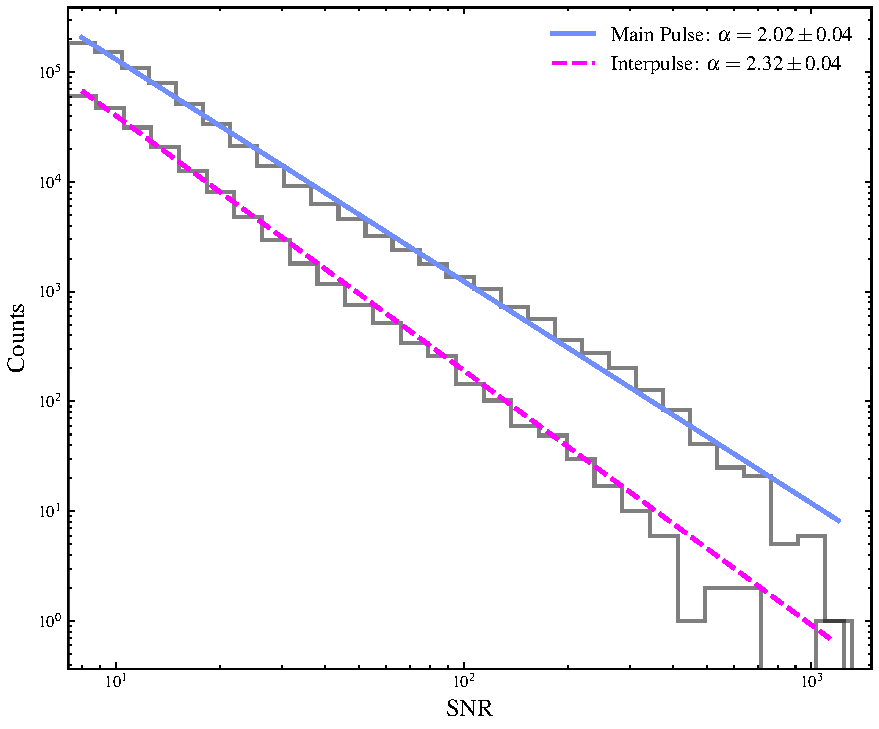
\includegraphics[width=0.65\linewidth]{chapter4/figures/CrabGP_SNR_histogram.pdf}
%     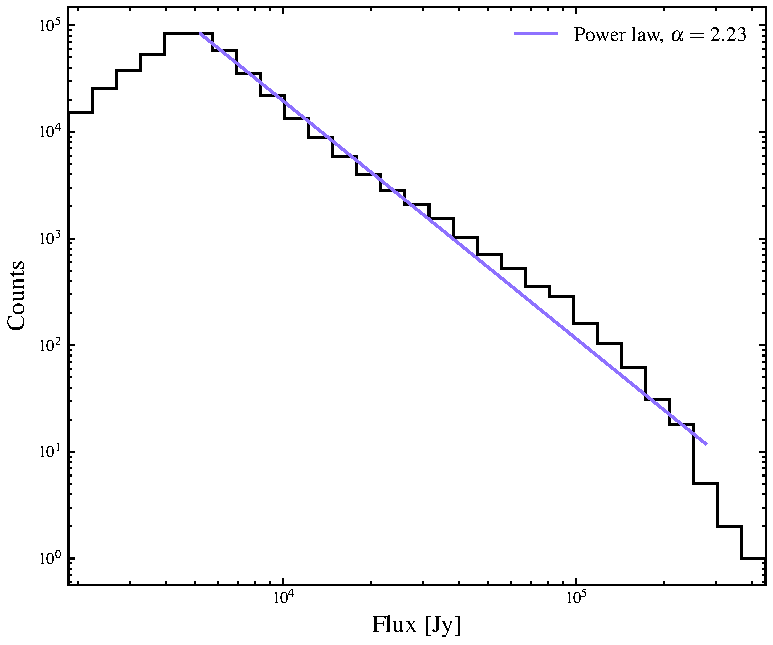
\includegraphics[width=0.65\linewidth]{chapter4/figures/CrabGP_Flux_histogram.pdf}
%     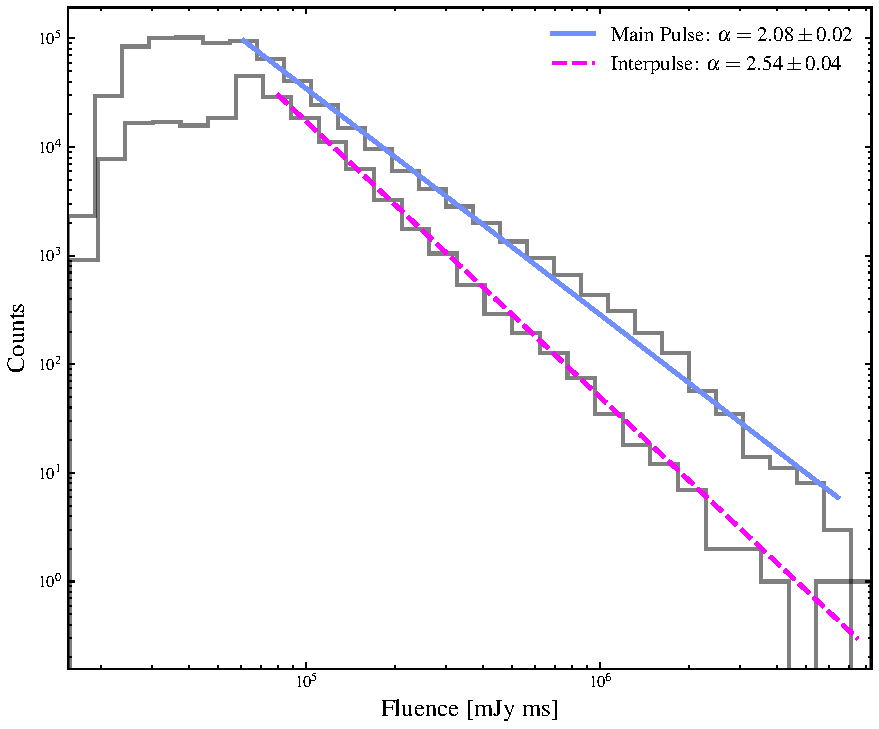
\includegraphics[width=0.65\linewidth]{chapter4/figures/CrabGP_Fluence_histogram.pdf}
%     \caption{The peak flux density distribution of observed giant pulses fitted to a power law.}
%     \label{fig:SNR_histogram}
% \end{figure}

\begin{figure}[h]
    \centering
        \begin{minipage}{0.48\linewidth}
        \centering
        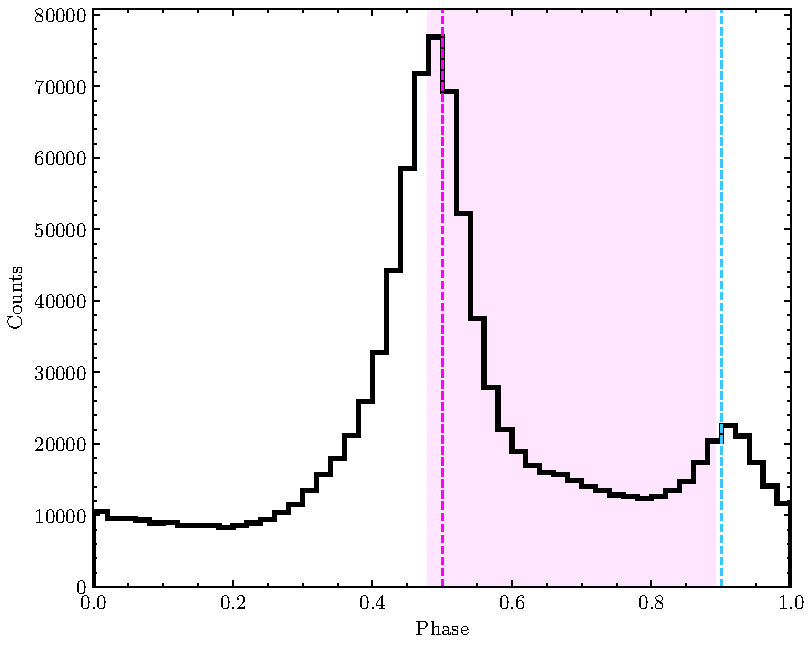
\includegraphics[width=\linewidth]{chapter4/figures/CrabGP_Phase_histogram.pdf}
        % \captionsetup{labelformat=empty}
        \caption*{(a)}
    \end{minipage}
    \hfill
    \begin{minipage}{0.48\linewidth}
        \centering
        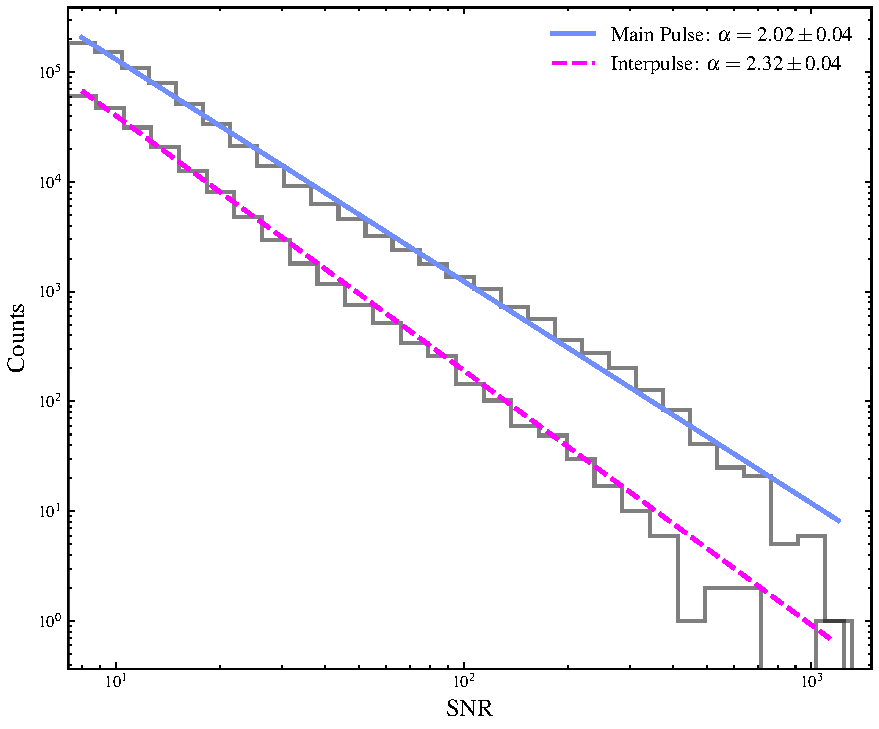
\includegraphics[width=\linewidth]{chapter4/figures/CrabGP_SNR_histogram.pdf}
        % \captionsetup{labelformat=empty}
        \caption*{(b)}
    \end{minipage}
    \vspace{0.5cm}
    \hfill
    \begin{minipage}{0.48\linewidth}
        \centering
        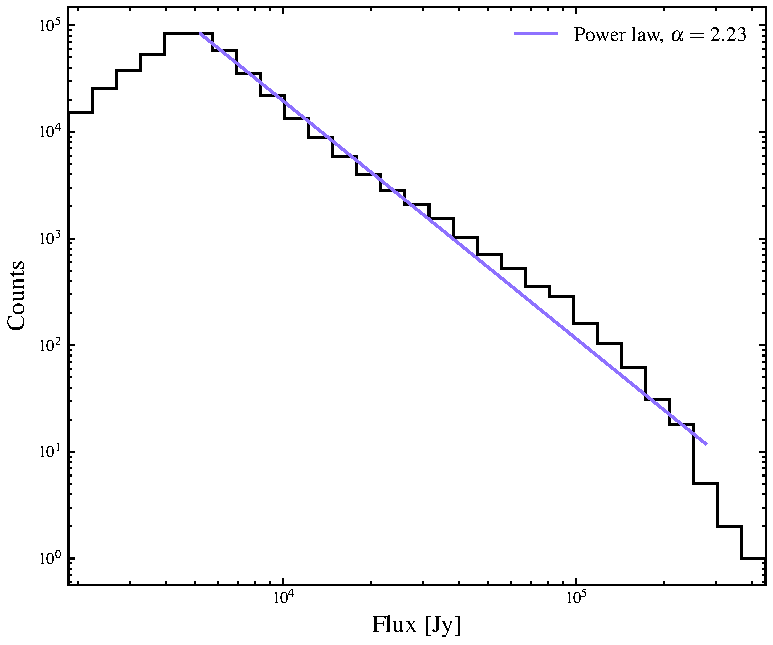
\includegraphics[width=\linewidth]{chapter4/figures/CrabGP_Flux_histogram.pdf}
        % \captionsetup{labelformat=empty}
        \caption*{(c)}
    \end{minipage}
    \begin{minipage}{0.48\linewidth}
        \centering
        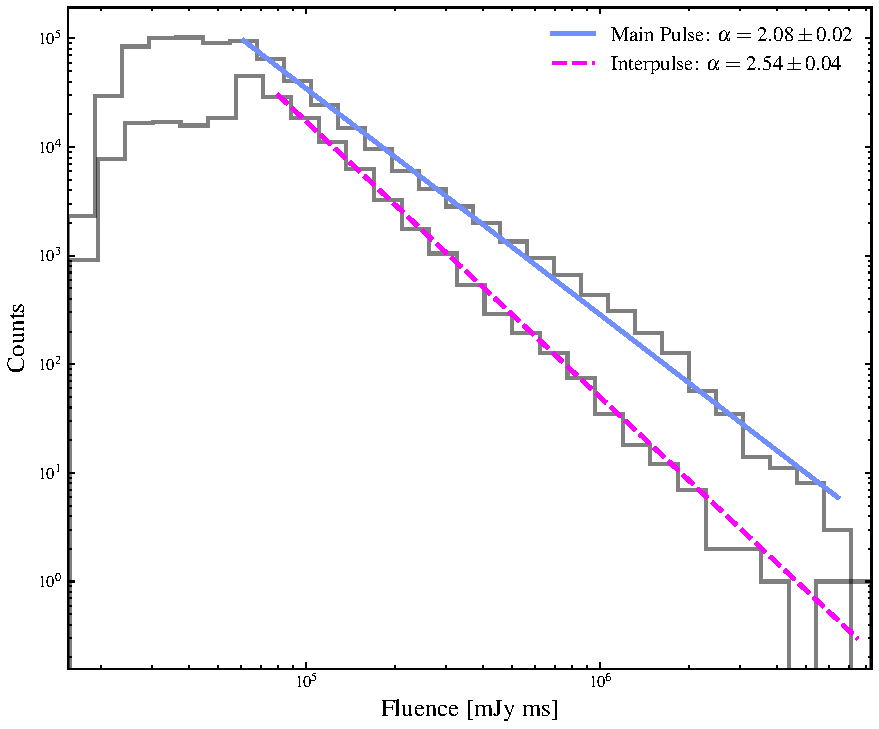
\includegraphics[width=\linewidth]{chapter4/figures/CrabGP_Fluence_histogram.pdf}
        % \captionsetup{labelformat=empty}
        \caption*{(d)}
    \end{minipage}

    \caption[Properties of the detected Crab pulses]{Properties of the detected Crab pulses.\textit{a)}:  pulse phase distribution. \textit{b)}: signal-to-noise ratio distribution. \textit{c):} flux distribution. \textit{d):} fluence distribution.}
    \label{fig:SNR_histogram}
\end{figure}

    % \caption{Properties of the detected Crab pulses. Top left:  pulse phase distribution.  Top right: signal-to-noise ratio distribution. \textit{Bottom left:} flux distribution.\textit{Bottom right:} fluence distribution.}

The details of the population of observed bursts from each day are shown in table \ref{tab:bursts}.

% \begin{figure}[h]
%     \centering
%     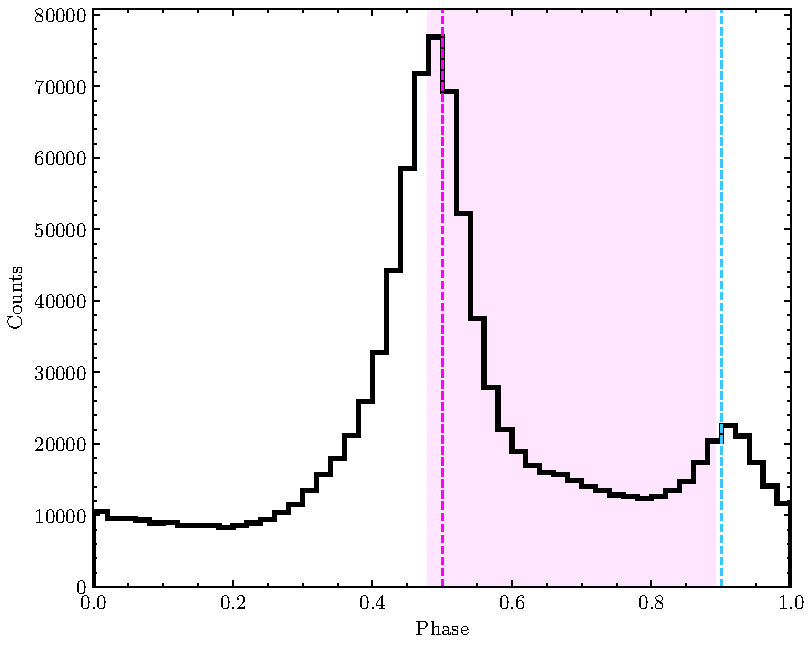
\includegraphics[width=0.65\linewidth]{chapter4/figures/CrabGP_Phase_histogram.pdf}
%     \caption{Caption}
%     \label{fig:placeholder}
% \end{figure}

\subsection{Fluence Measurement}

Fluence, $\mathcal{F}$, for each pulse detected above the noise floor. For pulses with SNR $>$ 100 the fluence was calculated using the scattering timescale. For pulses that didn't meet this threshold, the determined boxcar width and SNR obtained from \textsc{TransientX} was used such that $\mathcal{F} = \sqrt{W} \cdot S_{\text{burst}}$, similar the scattering timescale was used for pulses where scattering was measured. For each sub-band the best fit model was taken to be the best representation of the timescale for that specific pulse and the values were then averaged. 

% \begin{equation}
%     I(t) = \int_{-\infty}^{s} A \exp\left(-\frac{(t-s)^2}{2\sigma^2}\right) \exp\left(-\frac{s}{\tau}\right) H(s) \, ds
%     \label{eq:convolved}
% \end{equation}

% Here $A$ is the amplitude, $\sigma$ is the Gaussian instrumental width, $\tau$ is the intrinsic exponential decay timescale, $t$ is observation time relative to pulse peak, $s$ is the dummy variable for intrinsic emission time, and $H(s)$ is the Heaviside step function (emission only for $s\geq 0$). The total fluence of a pulse is then given by, 

% \begin{equation}
%     \mathcal{F} = \int_{t_{\min}}^{t_{\max}} I(t) \, dt
%     \label{eq:fluence}
% \end{equation}

Computing\footnote{\url{https://github.com/OwenJohnsons/Crab-Giant-Pulses/tree/main/modelling}} the fluence for each pulse gives an average fluence of $82.08~ \text{kJy~ms}$. The distribution of fluences for observed pulses is shown in the bottom right of \cref{fig:SNR_histogram}. 
% \subsection{Dispersion Measure}

% The DM of each

\begin{figure}
    \centering
    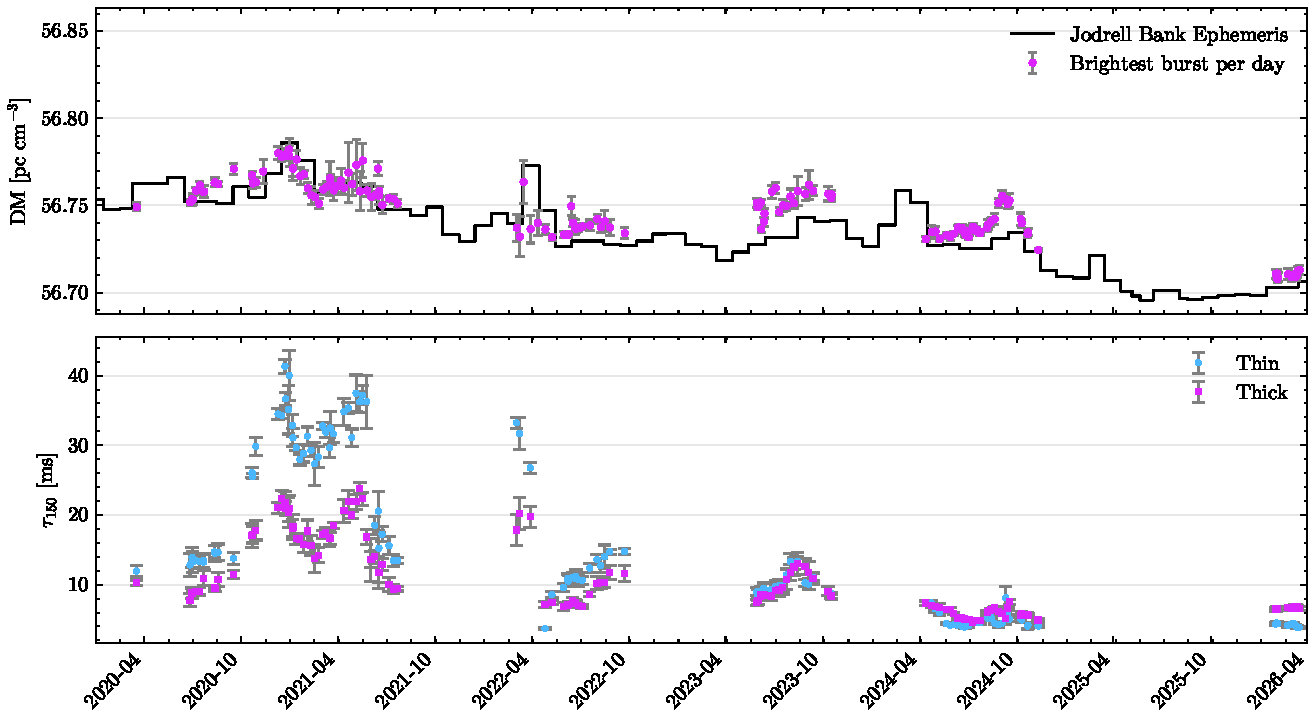
\includegraphics[width=0.94\linewidth]{chapter4/figures/scattering_and_DM.pdf}
    \caption[DM and scattering time series]{The \textit{top} panel shows the measured DM from 6 years of I-LOFAR data compared with ephemeris measured by Jodrell bank \citep{lyne_23_1993}. Whereas the \textit{(bottom)} shows the modelled scattering timescale for both the thick and modified thin screen models for each epoch during the observation campaign} 
    \label{fig:scatteringtDMtimeseries}
\end{figure}

\subsection{Pulse Distributions}

\Cref{fig:SNR_histogram} shows the distributions of pulses across phase, SNR and flux and fluence. The resultant distribution when first fitting the sample showed a bump towards the tail of the distribution. This bump is more pronounced in the flux distribution but present in all three. Initially this was thought to be the contribution of two different population with two different representative power-laws. The main pulse (MP) and the inter-pulse (IP), the MP is the dominant emission component and the IP is the secondary `bump' in the pulse profile shown in \cref{fig:foldedprofile} and \cref{fig:SNR_histogram} (a). The IP is usually treated as a distinct magnetospheric emission component that peaks around 0.9 in phase. It is probably linked to the opposite pole or outer magnetosphere, although its high-frequency behaviour suggests a more complex geometry than the standard two-pole picture \citep{cordes_brightest_2004, petrova_physics_2008}. 

In lieu of each burst was separated into either a population of MP or IP based on the calculated phase. MPs were considered the population that fell into the pink region in \cref{fig:SNR_histogram} (a) and IPs anywhere outside this region. The bump remained after the populations had been seperated out (what's shown in \cref{fig:SNR_histogram}) with the fitted slopes differ between the main pulse and interpulse populations, with the interpulse appearing systematically steeper in all three cases.

There is a likelihood that there is a genuine difference in burst statistics between the two pulse windows. However, it could also reflect selection effects, incomplete phase tagging, and scattering-related smearing that makes the bright end of the sample harder to interpret cleanly. The scattering present in the Crab pulses at these lower frequencies makes it that the pulse broadening makes the exact pulse phase hard to determine as observed arrival times will be shifted from the point of their intrinsic emission. 

A way to account for this could be the use of cyclic spectroscopy. Cyclic spectroscopy is a coherent folding technique that recovers phase‑preserving, high‑resolution frequency information by exploiting pulsar periodicity; it allows estimation and (where feasible) de-convolution of the ISM impulse response so that intrinsic pulse phase structure can be recovered and scattering‑induced broadening corrected \citep{demorest_cyclic_2011, turner_constraining_2026}. This would make it easier to discern the true phase of the single pulses, as it stands the phase boundary is too `fuzzy' for a sharp seperation in the pulse populations. 

A further potential contribution to consider the higher S/N pulses may be bias as the fitted scattering timescale is easier to discern from the noise floor causing pulses in with a higher S/N have a more representative fluence and flux to the low S/N population. Overall the current results are therefore best interpreted as suggestive, but not as a definitive measurement of intrinsic pulse-phase or fluence boundaries between IP and MP population and the Crab as a whole. 

A power law, $Ax^{-\alpha}$, was fitted by performing a weighted ($\sqrt{N}$) least-squares fit in logarithmic space. Parameter uncertainties were estimated from the covariance matrix returned by the weighted linear regression, taken as the square root of the diagonals in the covariance matrix, $\sqrt{\rm{Cov}(c,c)}$. The fitted power‑law indices for SNR, flux and fluence in our Crab giant‑pulse sample (MP $\sim$2.0–2.1; IP $\sim$ 2.4–2.8) are consistent with previously published ranges for Crab GPs, which typically report indices between 1.6–3.6 at these frequencies depending on the chosen observable \citep{karuppusamy_giant_2010, karuppusamy_crab_2012, sokolowski_100_2025}.  The spread in fitted power-law indices reflects differences in observing frequency, observable definition, fit range, completeness, and scattering bias which has been showcased here. As a result there is no universally accepted but rather an expected range based on frequency, chosen subband and so on.  

\subsection{Scattering}

As previously discussed scattering was fitted to each of the GPs above an SN of 100 after using \textsc{DM\_phase}. In observations where no GP greater than 100 was observed, the next brightest pulse was used. As described in §\ref{sec:modelScattering} both modified thin (eq. \ref{eq:thin_model_mod}) and thick (eq. \ref{eq:thick_model}) models was fitted to the data and their statistical significance noted. The scattering timescale in each sub-band of each pulse was measured, the median scattering value was taken for both the thin and thick scattering models and a power law in the following form.

\begin{equation}
    \tau(f) = \tau_{\mathrm{150}} \left[\frac{f}{150~\text{MHz}} \right]^\alpha
    \label{eq:powerlawscattering}
\end{equation}

\Cref{eq:powerlawscattering}  was then fit to the median sub-band values using non-linear least squares optimisation. Here $\tau_{150}$ is the scattering timescale scalled to 150~MHz and $\alpha$ is the scattering index. The resultant values for each epoch are shown in \cref{fig:scattering} where the errors where errors in this case are estimated from the covariance matrix for each fit. 

The measured scattering parameters when compared to the DMs allow for an analysis of the relationship between DM accuracy and the pulse broadening due to scattering. The values for each GP where scattering was modelled is shown in \cref{fig:DMoffset} against the relative offset of the nearest Jodrell Bank ephemeris where the colour represents the centre frequency of the subband. 

The lower the observing frequency the better the delineation of DM as dispersion delay increases as with $f^{-2}$, in theory improving the accuracy of the determined DM. However, at these frequencies scattering is also substantially increased $\sim f^{-4}$, leading to large broadening in the observed pulse, as observed in \cref{fig:scattering}. Consequently, a trade-off arises in the ability to measure DM and the increased temporal offset that comes with scattering.  

To quantify the trade-off the values obtained for the scattering power law, \cref{eq:powerlawscattering} was compared against the dispersive delay introduced by a finite DM uncertainty, $\sigma_{\mathrm{dm}}$ across the observed bandwidth. The `transition' frequency was estimated by equating the scattering timescale with the DM dispersion delay across the band, 

\begin{equation}
    \tau (f) = \mathcal{D} \cdot \sigma_{\text{DM}} \left[ \left( f - \frac{\Delta f}{2}\right)^{-2} -\left( f +\frac{\Delta f}{2}\right)^{-2} \right] 
    \label{eq:scat_dm}
\end{equation}

\Cref{eq:scat_dm} suggest that although very low frequencies provide strong dispersive sensitivity, the rapidly increasing scattering ultimately limits the achievable DM precision from single Crab GPs. Similarly, at sufficiently high frequencies the scattering becomes negligible but DM sensitivity also diminishes. 

\begin{figure}
    \centering
    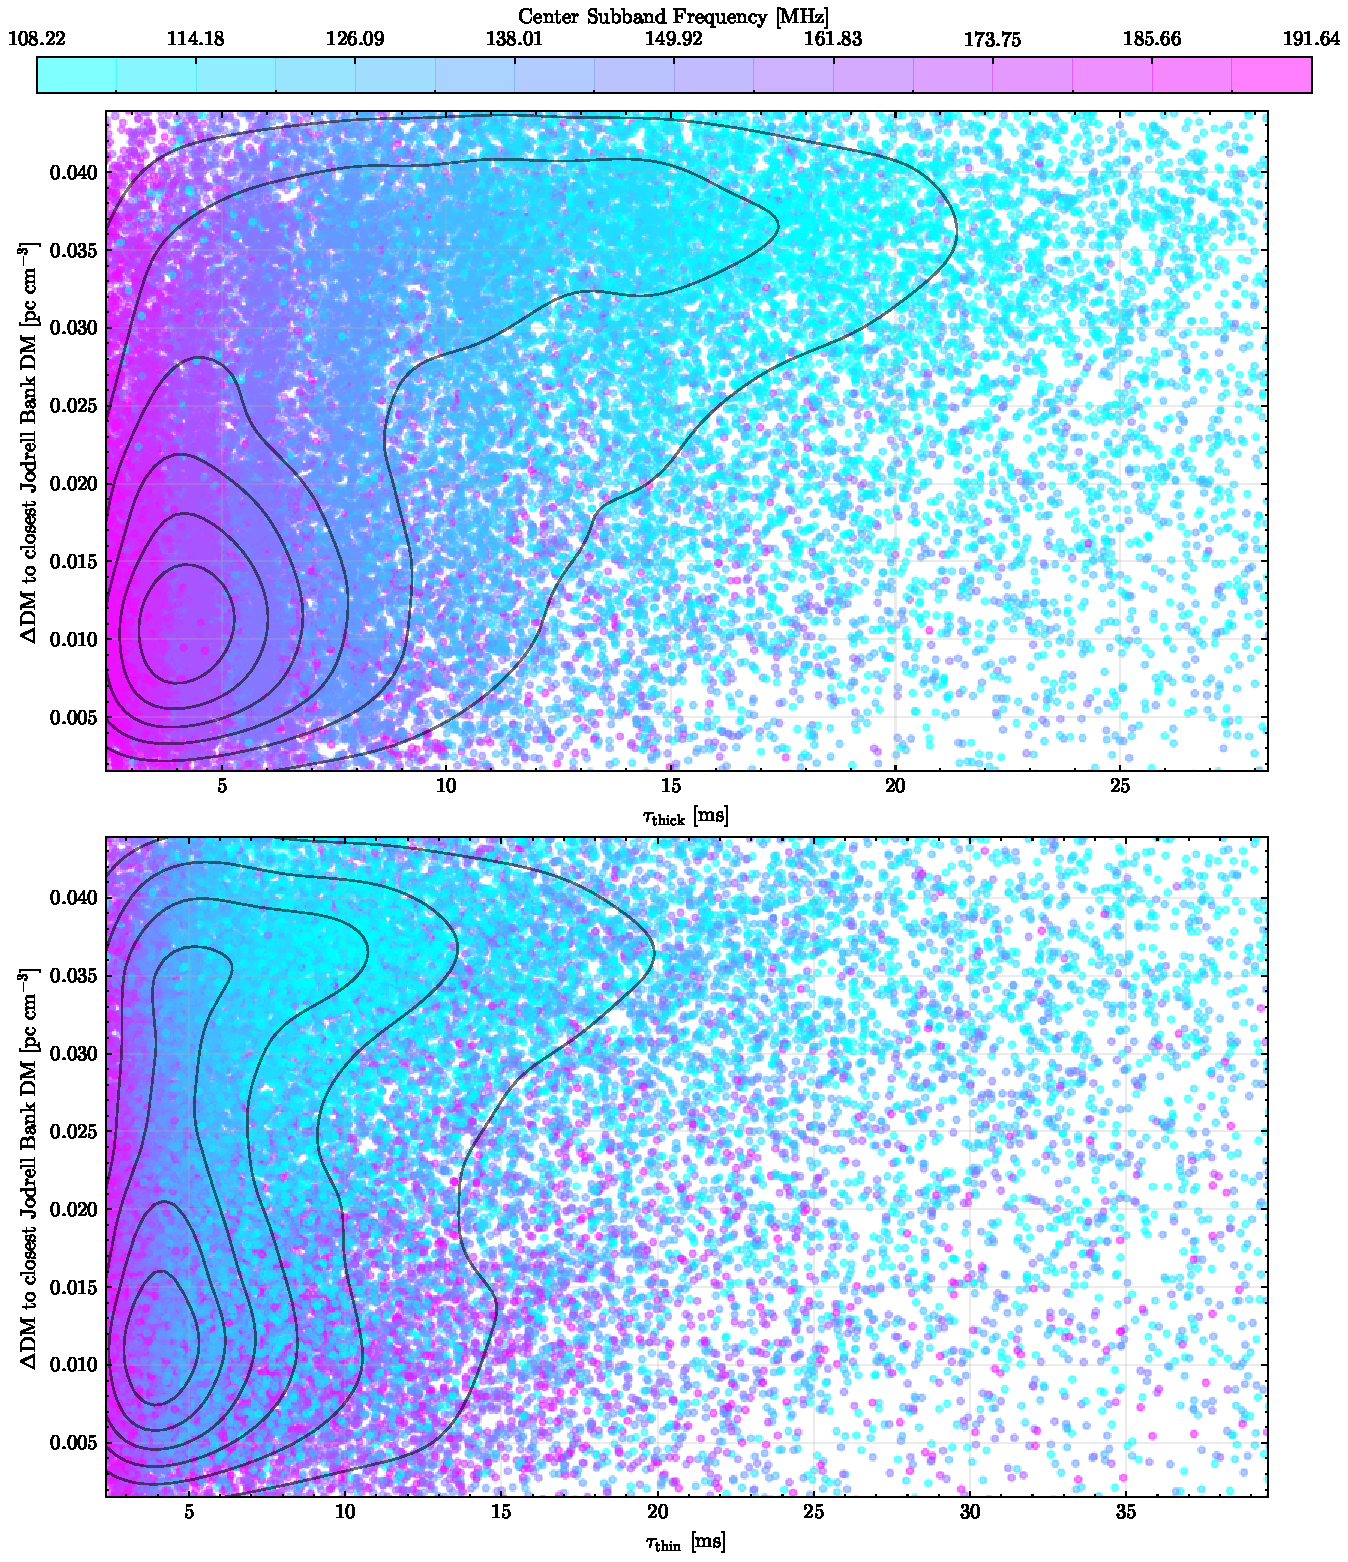
\includegraphics[width=0.95\linewidth]{chapter4/figures/DMoffset_contours.pdf}
    \caption[The DM offset of each pulse relative to the nearest measured reference DM ]{The DM offset of each pulse relative to the nearest measured DM from Jodrell Bank ephemeris plotted against the thick screen \textit{(top)} and modified thin screen \textit{(bottom)} scattering models. Each point corresponds to a measured scattering time of a burst with colour corresponding to the centre frequency of the subband.}
    \label{fig:DMoffset}
\end{figure}



\subsection{Implications on the Crab Nebula}

As previously discussed, scattering timescales and dispersion measure are not independent observables. The scattering variability coupled with the offsets of DMs measured of the single pulses in comparison to the Jodrell Bank ephemeris making it difficult to reliably distinguished true variation in DM. The time series itself regardless suggests that there are structures in the Crab nebula itself that vary significantly on small timescales (i.e. 2020-10 to 2021-04). As already mentioned as a possible solution is to use pulsar cyclic spectroscopy \citep{demorest_cyclic_2011,dolch_deconvolving_2021,turner_constraining_2026}. As the ISM is treated as a linear transfer function that convolves the intrinsic pulsar voltage signal, then uses the pulsar’s periodic coherence to estimate and de-convolve the ISM response from the observed voltages. This would be difficult due to the temporal variations in the local nebula itself, but may correct enough of the scattering that the DM precision improves sufficiently enough to further model the local nebulas electron content. 

\begin{figure}[h]
    \centering
    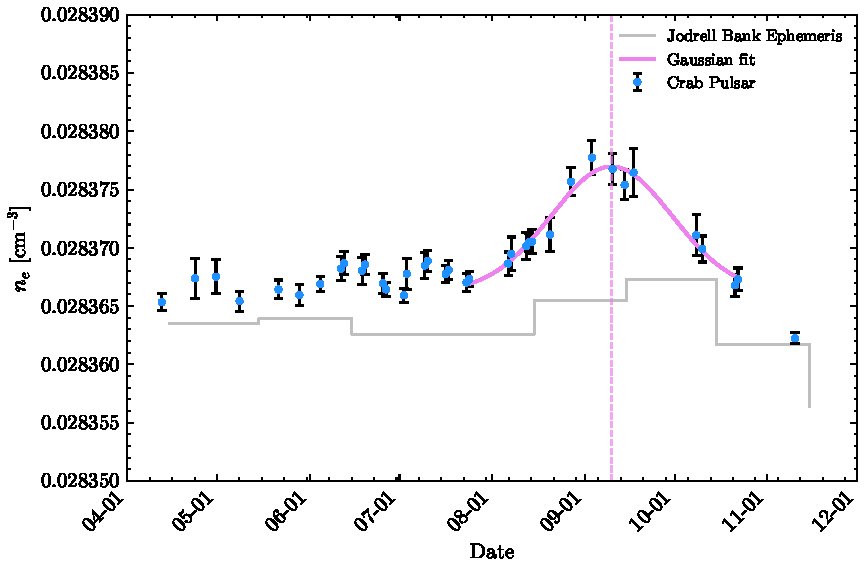
\includegraphics[width=0.75\linewidth]{chapter4/figures/nebulaMovement_ne.pdf}
    \caption[Electron density, $n_e$ as a function of time.]{Electron density, $n_e$ as a function of time. With a Guassian fitted shown in pink and Jodrell bank Ephemeris shown in grey.}
    \label{fig:datevsNe}
\end{figure}

Taking the period of the distinct rise shown in \cref{fig:scatteringtDMtimeseries} from around September to November and plotting the average electron content as a function of time and fitting a Gaussian an estimate can be made to the transverse time of a filament along the LOS between the observer and the Crab assuming that the main contributions come of DM variations come from the clump itself and not the background electron density. 

Using the fitted Gaussian width as a crossing time as the filament the transverse velocity can be estimated as $v_\perp \approx L/\Delta t$, where $L$ is the width of the filament and $\Delta t$ is taken to be the Gaussian FWHM, 2.355 $\sigma$ where, $\sigma =20.22~\rm days $ which gives a $\Delta t \approx 47.6$ days.  \cite{arias_crab_2025} measure state the Crab filament core resolves at $\sim 0.03$ pc for the dense cores and $\sim 0.08-0.2$ pc for the broader diffuse envelope component. The value for $L$ then depends on whether the observed DM rise as whether that is indicative of a compact core filament or an extended absorbing envelope, in this case the density change from baseline to peak is $\sim 0.4\% $ are far below the reported densities of the Crab's filaments \citep{arias_crab_2025}, this points to the contribution being instead from a diffuse plasma. In any case using the values listed above for $L$ the transverse velocity yield a value of $190-380~\rm{km~s}^{-1}$ which is consistent with expected values for Crab filament and ejecta proper motion \citep{trimble_motions_1968}. 

Taken together these constraints imply that DM excursion doesn't arise from the compact high-density filament core in the immediate vicinity of the pulsar and the envelope filaments are too far away to effect the line of sight. This is evidence that favours an origin more extended in a Rayleigh-Taylor-shaped filamentary ejecta. Further variations measured over time can rule out some nearby, compact plerionic\footnote{plerion - a filled-centre supernova remnant} structures and instead use the duration to place upper limits on the size and total emitting material of candidate filaments or wisps. 



%So here a range of $L = 0.03-0.04$ for the more extended absorbing envelope



% 0.15970000000000084
% 2020-03-17 19:14:21.408557 2026-03-17 19:39:34.264415
% Gaussian peak date: 2024-09-09 21:24:52.941136
% Gaussian sigma: 20.22 days


\subsection{Implications on the Solar Wind}

Probing the Sun with GPs over long timescales prove to be more difficult, while some GPs can be clearly can be seen during radio solar bursts as shown in \cref{fig:GPthroughBurst}, the precision needed to probe the electron content from the Sun is on the order of $10^{-3}-10^{-4}$~\dm \citep{tiburzi_impact_2021, susarla_exploring_2024} the variations in the Crab nebula itself aren't constrained enough to making any meaningful long-term conclusions on the sun's electron content using GPs. As expected the number of observed bursts decreases with solar elongation (see table \ref{tab:bursts}).  

\begin{figure}
    \centering
    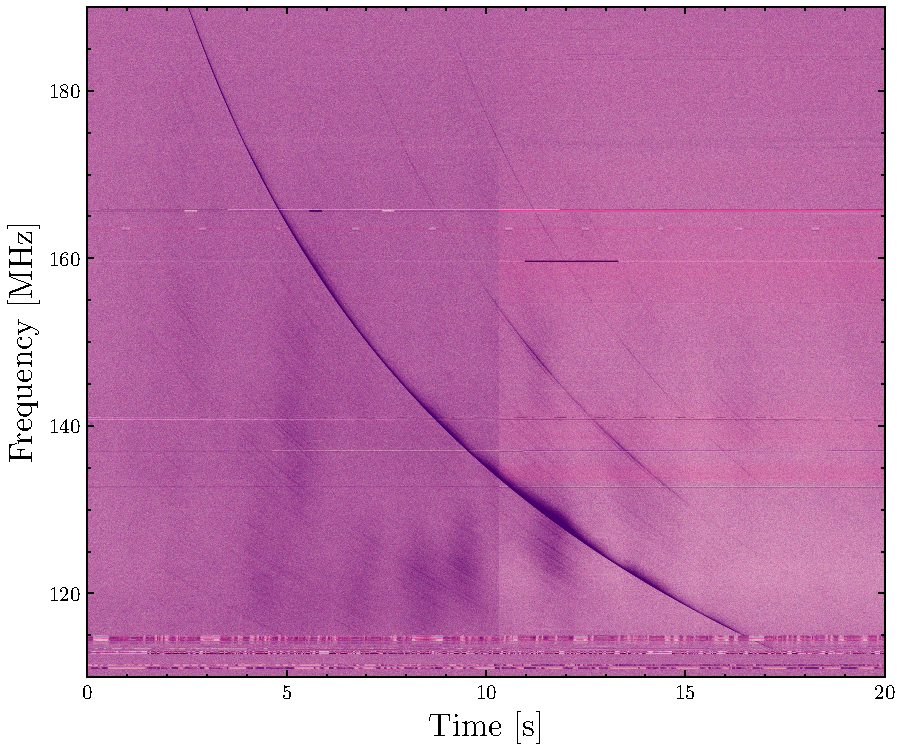
\includegraphics[width=0.9\linewidth]{chapter4/figures/Crab_raw_native_5s.pdf}
    \caption[Dispersed waterfall of several GPs through ionospheric disturbance]{Dispersed waterfall of several GPs observed during the 30th of June 2020 with a solar separation of $14.9^\circ$ from beam bore sight with ionospheric scintillation present. The most prominent burst had an S/N of 1720.1 with a DM of $56.754 \pm 0.003$ \dm. }
    \label{fig:GPthroughBurst}
\end{figure}

\section{Conclusion \& Future Work} \label{sec:conclusion}

This work presents a six year observing campaign of the Crab pulsar using I-LOFAR. The dataset is comprised over a million single pulses and half a million giant pulses. The exceptional brightness of the Crab pulsar allowed for measurement of both dispersion measure and the pulse broadening due to scattering along the line of sight for over 5000 pulses above an S/N of 100.

A DM time series was created using both single pulse phase coherent DM optimisation and timing through folding. It was found that apparent DM offsets can arise from frequency-dependent pulse broadening rather than genuine changes in the DM, making it difficult to determine any variation in the local nebula on short timescales in comparison to other higher frequency Crab observations. Although lower frequencies provide enhanced sensitivity to small DM offsets, the rapidly increasing scattering broadens the pulse profile sufficiently to limit the achievable DM precision from individual giant pulses.

The measured DM and scattering variations further suggest that the Crab Nebula is highly dynamic on observable timescales, with turbulent or filamentary structures contributing significantly to the observed propagation effects. It was also determined that the local variations in the nebula aren't well enough constrained to be able to `untangle' DM changes caused by the sun when the Crab was close to the ecliptic. 

Analysis of the giant-pulse population showed that the measured S/N, flux and fluence distributions follow power-law behaviour consistent with previous studies of the Crab pulsar. Although the main-pulse population doesn't exhibit a small bump in its distribution not completely following a power law. This is primarily attributed to the difficulty of pulse separation of the two populations due the effects of scattering.

Combining the long-term DM and scattering measurements also enabled a discussion on the potential constraints that low frequency observations could place n the local Crab environment. The duration and magnitude of the observed DM enhancement are consistent with a diffuse filamentary or Rayleigh-Taylor ejecta structure crossing the line of sight. Although the exact electron-density distribution cannot yet be uniquely determined, these measurements demonstrate the potential of long-term low-frequency giant-pulse monitoring to probe the evolving plasma environment surrounding the Crab pulsar.

Overall, this work demonstrates that giant pulses from the Crab pulsar at low frequencies as one of the most powerful probes intervening medium along the line of sight. Although scattering presently limits the achievable DM precision at LOFAR frequencies. The continued long-term monitoring and simultaneous observations at higher frequencies will provide a more complete picture of the evolving electron content of the Crab Nebula and improve our understanding of pulse propagation through complex plasma environments.